%% ============================================================
%%  BSAAP: Blockchain-Integrated Secure Agent-to-Agent
%%  Authentication Protocol for Multi-Agent AI Systems
%%  Journal of Systems Architecture (Elsevier)
%%  ISSN 1383-7621  |  elsarticle two-column, 5p, times
%%  All references verified against uploaded source documents.
%% ============================================================
\documentclass[review,5p,twocolumn,times]{elsarticle}

%% Core packages
\usepackage{amsmath,amssymb,amsfonts}
\usepackage{algorithm}
\usepackage{algpseudocode}
\usepackage{graphicx}
\usepackage{tikz}
\usetikzlibrary{shapes,arrows.meta,positioning,fit,calc,
                decorations.pathreplacing,backgrounds}
\usepackage{pgfplots}
\pgfplotsset{compat=1.18}
\usepackage{pgfplotstable}
\usepackage{booktabs,multirow,tabularx}
\usepackage{float}
\usepackage[hidelinks]{hyperref}
\usepackage{cleveref}
\usepackage{listings,xcolor}
\usepackage{microtype}
\usepackage{url}
\usepackage{siunitx}
\usepackage{amsthm}
\renewcommand{\qedsymbol}{}

%% Theorem environments
\newtheorem{theorem}{Theorem}[section]
\newtheorem{definition}{Definition}[section]
\newtheorem{proposition}{Proposition}[section]

%% Listings style
\definecolor{codebg}{rgb}{0.97,0.97,0.97}
\definecolor{codestr}{rgb}{0.13,0.47,0.13}
\definecolor{codecomment}{rgb}{0.4,0.4,0.4}
\definecolor{codekw}{rgb}{0.10,0.10,0.60}
\lstset{
  backgroundcolor=\color{codebg},
  basicstyle=\ttfamily\scriptsize,
  keywordstyle=\color{codekw}\bfseries,
  stringstyle=\color{codestr},
  commentstyle=\color{codecomment}\itshape,
  breaklines=true, frame=single, numbers=left,
  numberstyle=\tiny\color{gray},
  xleftmargin=0.5em, xrightmargin=0.3em,
}

\journal{Journal of Systems Architecture}

%% TikZ styles
\tikzset{
  ebox/.style={rectangle,draw,rounded corners=3pt,
               minimum width=1.5cm,minimum height=0.55cm,
               font=\scriptsize,align=center,fill=blue!8},
  chainbox/.style={rectangle,draw,fill=orange!18,rounded corners=2pt,
                   minimum width=1.5cm,minimum height=0.5cm,
                   font=\scriptsize,align=center},
  arr/.style={-{Stealth[length=4pt]},thick},
  darr/.style={-{Stealth[length=4pt]},dashed,gray!70},
}

\begin{document}

%% Front matter
\begin{frontmatter}

\title{Blockchain-Integrated Secure Agent-to-Agent Authentication Protocol
       for Multi-Agent AI Systems (BSAAP)}

\author[gim]{Karthik V.}

\address[gim]{Goa Institute of Management, Sanquelim, Goa~403505, India.
  M.Tech AI/ML, SRIP-2026 Big Data Analytics Research Fellow.}

\begin{abstract}
The rapid proliferation of large-language-model-based autonomous agents that
communicate, delegate tasks, and share resources has exposed a critical
security vacuum: existing authentication frameworks---PKI, OAuth~2.0, and
JSON Web Tokens---were designed for human users or static microservices and
are architecturally ill-suited to the dynamic, ephemeral, and autonomous
nature of modern multi-agent systems (MAS). We present the
\emph{Blockchain-Integrated Secure Agent-to-Agent Authentication Protocol}
(BSAAP), a six-stage cryptographic protocol providing mutual authentication,
capability-scoped access control, forward-secret session key establishment,
and auditable accountability for autonomous agent interactions. BSAAP is
designed to anchor agent identity on a Hyperledger Fabric permissioned ledger
via W3C Decentralised Identifiers (DID), enforce smart-contract revocation,
and chain every session record in a Merkle audit log; the current prototype
implements the Fabric layer in simulation mode with an in-memory ledger. The
protocol employs ECDSA P-256 for long-term identity signatures, X25519
ephemeral Diffie-Hellman for forward-secret session keys, AES-256-GCM for
authenticated payload encryption, and HKDF-SHA-256 for key derivation.
Empirical evaluation over 100 repeated trials on a standard hardware testbed
yields a mean full-authentication latency of $1.118 \pm 0.279$~ms,
certificate verification in $0.154 \pm 0.024$~ms, and 100\% detection across
all five threat-model attack classes. Formal security analysis is provided via
an ROR-model reduction bounding the adversarial advantage by two times the
ECDDH advantage plus a negligible birthday-bound term (Theorem~\ref{thm:ror}),
four formal theorems, and AVISPA/HLPSL verification of the challenge-response
stages (Stages~2--3) returning \textsc{safe}. BSAAP is, to our knowledge,
the first agent-to-agent authentication protocol that unifies mutual
cryptographic identity binding, fine-grained capability scoping, ledger-backed
revocation, and hash-chained audit within a single formally analysed framework.
\end{abstract}

\begin{keyword}
Agent-to-Agent Authentication \sep Multi-Agent AI Systems \sep
Blockchain Trust Registry \sep Hyperledger Fabric \sep ECDSA P-256 \sep
X25519 ECDH \sep AES-256-GCM \sep Challenge-Response Protocol \sep
Zero-Trust Architecture \sep Decentralised Identifiers
\end{keyword}

\end{frontmatter}

%% ============================================================
\section{Introduction}\label{sec:intro}
%% ============================================================

The deployment of large-language-model (LLM)-based autonomous agents has
transformed software architecture. Platforms such as AutoGen, LangChain, and
CrewAI routinely orchestrate pipelines in which an \emph{orchestrator} agent
decomposes user goals and dispatches subtasks to specialist \emph{worker}
agents that may themselves invoke further agents or external APIs
\cite{wang2023survey}. Xu~et~al.\ report that CrewAI has executed more than
60 billion agent runs in total, with over 100\,000 multi-agent execution
groups processed each day \cite{agentdid2026}; Gartner projects that agentic
AI will autonomously resolve 80\% of common customer service issues without
human intervention by 2029 \cite{gartner2025agentic}.

\subsection{Motivation and Problem Statement}

In such ecosystems the security of inter-agent communication channels is
critical: a compromised or impersonated agent can corrupt task outputs,
exfiltrate sensitive data, or trigger unauthorised actions at enterprise
scale. Yet authentication in multi-agent AI systems remains immature.
Classical PKI \cite{rfc5280} targets human-operated server entities;
OAuth~2.0 \cite{rfc6749} addresses delegated human-to-service authorisation;
JSON Web Tokens \cite{rfc7519} provide stateless human session claims.
None of these frameworks accounts for the four defining characteristics of
autonomous AI agents: \emph{(i)} ephemeral instantiation and termination,
\emph{(ii)} decision-making identity (the agent acts on its own behalf),
\emph{(iii)} dynamic capability scope varying per task delegation, and
\emph{(iv)} the absence of a human operator to handle certificate prompts
or re-authentication flows.

Recent surveys confirm these gaps. A scan of approximately 2\,000 MCP
servers found that every single one lacked authentication \cite{aip2026}.
BlockA2A \cite{blocka2a2025} formally documents fragmented identity
frameworks, insecure communication channels, and the absence of immutable
audit trails as the three principal multi-agent security deficits.

We address these gaps with a targeted research question,
addressing the foundational security gap in multi-agent AI authentication:
\emph{How can we design a secure and
lightweight authentication protocol that allows one AI agent to verify the
identity, authority, and trustworthiness of another AI agent before
communication or task delegation?}

\subsection{Research Contributions}

BSAAP introduces five principal contributions:

\begin{enumerate}
  \item \textbf{On-chain agent DID registry (prototype in simulation):}
    Agent identity is designed to be anchored on
    a Hyperledger Fabric ledger via W3C DID Core \cite{w3c2022did}, making
    the trust registry tamper-evident and decentralised. The current prototype
    implements Fabric interactions via an in-memory simulation client.
  \item \textbf{Capability-scoped X.509 certificates:} Custom OID extensions
    encode each agent's allowed task scope, enabling fine-grained per-task
    authorisation without a centralised policy server.
  \item \textbf{ECDH-based forward-secret session keys:} Ephemeral X25519
    key exchange \cite{rfc7748} combined with HKDF-SHA-256 \cite{rfc5869}
    ensures that compromise of long-term keys cannot expose past sessions.
  \item \textbf{Smart-contract-enforced revocation (simulation):} Hyperledger
    Fabric chaincode is intended to enforce immediate credential revocation
    without CRL polling delays; the prototype validates this logic via
    simulated chaincode queries.
  \item \textbf{Merkle-chained audit trail (simulation):} Every session record
    is Merkle-linked and intended for on-chain commitment, providing an
    accountability trail verifiable by any authorised auditor.
\end{enumerate}

\subsection{Paper Organisation}

\Cref{sec:related} surveys related work across eight thematic clusters.
\Cref{sec:background} provides cryptographic preliminaries.
\Cref{sec:model} defines the system and threat model.
\Cref{sec:protocol} specifies all six BSAAP stages.
\Cref{sec:security} presents formal security analysis.
\Cref{sec:impl} describes the Python prototype.
\Cref{sec:eval} reports performance and security evaluation.
\Cref{sec:discussion,sec:limits} discuss findings and limitations.
\Cref{sec:conclusion} concludes.

%% ============================================================
\section{Related Work}\label{sec:related}
%% ============================================================

We survey existing work across eight thematic clusters and map each gap to a
specific BSAAP design decision.

\subsection{Agent Identity and DID Management (Cluster A)}

Xu~et~al.\ \cite{agentdid2026} introduced \emph{AgentDID}, which assigns
each AI agent a W3C DID anchored on the Ethereum ERC-1056 registry and
includes a context-consistency check to prevent identity misuse across tasks.
DID registration incurs 58\,238 gas (\$0.88, 15.37~s on Sepolia testnet);
full authentication latency averages $\approx$6.5~s due to blockchain
resolution overhead. Our protocol avoids this bottleneck entirely: the
permissioned Fabric ledger resolves registrations in $<1$~ms locally and
$<18$~ms in production endorsement. Lin~et~al.\ \cite{baid2025} proposed
\emph{BAID}, which binds identity to model-code integrity via zkVM-based
ERC-4337 on-chain registration, using the state-commitment
$h{=}H(S_t)$ and recursive proofs to defend against Sybil attacks. Neither
AgentDID nor BAID specifies an inter-agent challenge-response handshake;
this is exactly the layer that our Stage~2--3 design addresses.

\subsection{Token-Based Delegation and JWT Extensions (Cluster B)}

Goswami \cite{agenticjwt2025} proposed \emph{Agentic JWT} (A-JWT), a
dual-token scheme adding an \texttt{agent\_checksum} grant and Ed25519
Proof-of-Possession (PoP) keys to standard JWT, achieving sub-millisecond
verification overhead under a STRIDE threat model. A-JWT addresses single-hop
tool invocation but provides no blockchain anchor for revocation or
non-repudiation. South~et~al.\ \cite{stanford2025a2a} proposed
authenticated, authorised, and auditable delegation extending OAuth~2.0/OIDC
with agent cards and natural-language permission scopes; their work motivates
BSAAP's capability-scope OID extension.
Prakash \cite{aip2026} introduced \emph{AIP} and
Invocation-Bound Capability Tokens (IBCTs), which fuse identity, attenuated
authorisation, and provenance into an append-only Biscuit/JWT token chain.
AIP adds 0.22~ms overhead per real MCP call and detects 600/600 adversarial
attack attempts; however, it defines no blockchain-backed audit or formal
security proof. The on-chain tamper-evident audit and ROR-model security
reduction that AIP explicitly defers are central contributions of this work.

\subsection{Blockchain-Integrated Multi-Agent Security (Cluster C)}

Zou~et~al.\ \cite{blocka2a2025} proposed \emph{BlockA2A}, the first
systematic analysis of multi-agent trust vulnerabilities and a three-layer
framework comprising a DID identity layer, a Merkle-based ledger layer, and
a smart-contract enforcement layer. BlockA2A's Defence Orchestration Engine
(DOE) achieves sub-second counter-attack response (135~ms maximum). BSAAP
shares BlockA2A's blockchain anchoring philosophy but focuses on the
\emph{authentication protocol layer} (Stages~2--4) that BlockA2A omits,
providing formal cryptographic proofs and a precise key-establishment
specification absent from BlockA2A.

\subsection{Zero-Trust and ZKP-Enhanced IAM (Cluster D)}

Huang~et~al.\ \cite{zerotrust2025} proposed a zero-trust IAM framework for
agentic AI combining DIDs, Verifiable Credentials (VCs), ZKP-based
privacy-preserving attribute disclosure, and an Agent Naming Service (ANS)
under the MAESTRO umbrella. Their framework targets policy enforcement
at the enterprise level and does not specify a protocol-level handshake or
performance benchmarks. Our protocol-level handshake (Stages~2--4) is
designed to operate within such a zero-trust IAM layer.
NIST SP 800-207 \cite{nist2020zta}
and the BeyondCorp enterprise model \cite{ward2014beyondcorp}
mandate continuous verification of every request; the Stage-5 per-message
MAC check and per-session revocation query operationalise this principle
at the transport level.

\subsection{Capability Governance and Cryptographic Binding (Cluster E)}

Zhou \cite{govdyn2026} proved a Chain Verifiability Theorem and a Bounded
Divergence Theorem ($\varepsilon \leq 1{-}\alpha^{1/n}$) for AI agent
tool-use governance, instantiating two schemes: Ed25519/SHA-256 (97~$\mu$s)
and BBS+/Groth16 DV-SNARK (13.8~ms). The same capability-binding
principle is instantiated in our design at the certificate layer via X.509
OID extensions, making capability scope cryptographically inseparable from
agent identity.

\subsection{Provider-Mediated Governance (Cluster F)}

Syros~et~al.\ \cite{saga2026} presented \emph{SAGA}, a user-controlled
governance architecture published at NDSS 2026, employing one-time keys
(OTK) and Access Control Tokens (ACT) with ProVerif-proven mutual
authentication. SAGA evaluates a Provider-sharded architecture and achieves
formal proofs under a symbolic Dolev-Yao model.
Our design provides a complementary capability: a concrete cryptographic
specification for the initial handshake phase that SAGA delegates to
transport-layer TLS, together with blockchain-backed auditability that
SAGA's centralised Provider logs do not offer.

\subsection{Comparative Evaluation and Survey (Cluster G)}

A growing body of multi-agent security literature points to a common
conclusion: no single protocol jointly addresses the complete security
surface for autonomous agent authentication. Prakash \cite{aip2026}
notes that all 2\,000 MCP servers scanned lacked any form of authentication,
and BlockA2A \cite{blocka2a2025} identifies fragmented identity, insecure
channels, and missing audit trails as the three principal deficits. BSAAP
is designed to close the specifically identified gap: authenticated mutual
identity binding with blockchain-anchored audit for A2A protocols.

\subsection{Classical PKI and Challenge-Response Foundations (Cluster H)}

ISO/IEC 9798-3 \cite{isoiec9798} defines the theoretical basis for
BSAAP Stage~3 as a three-pass challenge-response protocol using public-key
signatures. ECDSA provable security was established by Fersch~et~al.\ 
\cite{fersch2016provable}, forming the basis of our mutual authentication
theorem. TLS~1.3 has been verified with ProVerif by Bhargavan~et~al.\ 
\cite{bhargavan2017tls13}; a similar model for the full six BSAAP stages is
identified as future work.

\begin{table*}[!ht]
\centering
\caption{Comparison of BSAAP with related agent authentication approaches.
  (\checkmark)~=~fully supported; ($\circ$)~=~partial; ($\times$)~=~absent.}
\label{tab:comparison}
\footnotesize
\setlength{\tabcolsep}{3.5pt}
\resizebox{\textwidth}{!}{%
\begin{tabular}{@{}p{2.5cm}p{1.3cm}p{2.0cm}ccccc@{}}
\toprule
\textbf{Work} & \textbf{Year} & \textbf{Auth Method}
  & \textbf{BC} & \textbf{Cap.}
  & \textbf{Proof} & \textbf{Agent-Spec.}
  & \textbf{Fwd.Sec.}\\
\midrule
AgentDID \cite{agentdid2026}       & arXiv'26  & DID+ERC-1056       & \checkmark & $\times$ & $\times$ & \checkmark & $\times$ \\
A-JWT \cite{agenticjwt2025}        & arXiv'25  & JWT+PoP            & $\times$ & $\times$ & $\times$ & \checkmark & $\times$ \\
BAID \cite{baid2025}               & arXiv'25  & zkVM+ERC-4337      & \checkmark & $\times$ & $\circ$ & \checkmark & $\times$ \\
Zero-Trust \cite{zerotrust2025}    & arXiv'25  & DID+VC+ZKP         & $\circ$ & \checkmark & $\times$ & $\circ$ & $\times$ \\
SAGA \cite{saga2026}               & NDSS'26   & OTK+ACT            & $\times$ & \checkmark & \checkmark & \checkmark & \checkmark \\
Gov.Cap. \cite{govdyn2026}         & arXiv'26  & Ed25519 bind       & $\times$ & \checkmark & $\circ$ & \checkmark & $\times$ \\
AIP \cite{aip2026}                 & arXiv'26  & IBCT/Biscuit       & $\times$ & \checkmark & $\times$ & \checkmark & $\times$ \\
BlockA2A \cite{blocka2a2025}       & arXiv'25  & DID+Merkle         & \checkmark & \checkmark & $\times$ & \checkmark & $\times$ \\
Stanford \cite{stanford2025a2a}    & arXiv'25  & OAuth+OIDC         & $\times$ & \checkmark & $\times$ & \checkmark & \checkmark \\
ISO 9798-3 \cite{isoiec9798}       & ISO'19    & Chall-Resp         & $\times$ & $\times$ & $\circ$ & $\times$ & $\times$ \\
\midrule
\textbf{BSAAP} (ours)         & 2026      & ECDSA+\allowbreak{}ECDH+\allowbreak{}BC & $\circ^\dagger$ & \checkmark & \checkmark & \checkmark & \checkmark \\
\bottomrule
\multicolumn{8}{@{}l@{}}{\scriptsize BC=Blockchain; Cap=Capability; Proof=Formal proof; Agent-Spec.=Agent-specific; Fwd.Sec.=Forward secrecy.}\\
\multicolumn{8}{@{}l@{}}{\scriptsize $^\dagger$Blockchain layer implemented in simulation mode; production support remains future work.}
\end{tabular}%
}% end resizebox
\end{table*}

%% ============================================================
\section{Background and Cryptographic Preliminaries}\label{sec:background}
%% ============================================================

\subsection{Digital Certificates and X.509 v3}

An X.509 v3 certificate \cite{rfc5280} is a signed data structure binding a
public key to an identity: $\mathsf{cert} = (\mathit{tbs}, \sigma_{\mathcal{CA}})$
where $\mathit{tbs}$ encodes subject DN, issuer DN, validity period,
$pk_{\mathit{subj}}$, and typed extensions.
BSAAP adds four custom OID extensions in the namespace
$1.3.6.1.4.1.99999.1.x$: \texttt{capabilityScope} (JSON array of allowed
task strings), \texttt{agentRole}, \texttt{agentDID}, and \texttt{trustLevel}.

\subsection{ECDSA P-256}

Let $\mathbb{G}$ be the SECP256R1 group of prime order $q$ with generator $G$
\cite{nistfips186}. Key generation: choose $d \xleftarrow{\$} \mathbb{Z}_q^*$;
compute $Q = dG$; return $(d, Q)$.
Signing message $m$: choose $k \xleftarrow{\$} \mathbb{Z}_q^*$;
compute $(r, s) = \bigl(x([k]G) \bmod q,\; k^{-1}(H(m)+dr) \bmod q\bigr)$.
Verification: check $r \equiv x\bigl([s^{-1}H(m)]G + [s^{-1}r]Q\bigr) \pmod{q}$.
Security rests on the ECDLP; provable unforgeability under the random oracle
model is established in \cite{fersch2016provable}.

\subsection{X25519 and ECDH Key Exchange}

X25519 \cite{rfc7748,bernstein2006curve25519} defines scalar multiplication on
Curve25519, a Montgomery curve over $\mathbb{F}_{2^{255}-19}$.
Given $a \xleftarrow{\$} \{0,1\}^{255}$ and $B = bG$, the shared secret is
$\mathsf{SS} = aB = abG$.
Security under the Decisional Diffie-Hellman (DDH) assumption \cite{diffie1976new}: no PPT
adversary distinguishes $abG$ from a random group element with non-negligible
advantage. BSAAP uses fresh ephemeral X25519 key pairs per session; private
keys are erased immediately after shared-secret computation.

\subsection{AES-256-GCM Authenticated Encryption}

AES-256-GCM \cite{nistsp800-38d} provides IND-CCA2-secure AEAD.
For key $K$ (256-bit), IV $N$ (96-bit), plaintext $P$, and associated
data $A$:
\begin{align}
\mathsf{GCM.Enc}(K,N,P,A) &\to (C, T), \nonumber\\
\mathsf{GCM.Dec}(K,N,C,T,A) &\to P \;\text{or}\; \bot
\label{eq:gcm}
\end{align}
$T$ is a 128-bit authentication tag; decryption returns $\bot$ if $T$ is
invalid. BSAAP sets $A = \mathsf{sid} \| \mathsf{seqNum}$ to bind the tag to
session and sequence context.

\subsection{HKDF-SHA-256}

$\mathsf{HKDF}$ \cite{rfc5869} is a two-stage key derivation function:
\begin{align}
\mathsf{PRK} &= \mathsf{HMAC\text{-}SHA256}(\mathsf{salt},\; \mathsf{IKM})
\label{eq:hkdf1}\\
K &= \mathsf{HMAC\text{-}SHA256}(\mathsf{PRK},\; \mathsf{info} \| \mathtt{0x01})
\label{eq:hkdf2}
\end{align}
BSAAP sets $\mathsf{IKM} = \mathsf{SS}$ (ECDH output),
$\mathsf{salt} = n_1 \| n_2$ (nonces from Stages~2 and~3), and
$\mathsf{info} = \texttt{"BSAAP-v1-session"}$.

\subsection{Hyperledger Fabric}

Hyperledger Fabric \cite{androulaki2018hyperledger} is a permissioned
distributed ledger with MSP-based identity, channel-based data isolation,
and deterministic chaincode execution achieving approximately 3\,000
transactions per second on standard hardware.
BSAAP uses a single channel (\texttt{bsaap-channel}) with six chaincode
functions: \texttt{RegisterAgent}, \texttt{RevokeAgent}, \texttt{IsRevoked},
\texttt{CreateSession}, \texttt{CloseSession}, and \texttt{WriteAuditRecord}.

\subsection{W3C Decentralised Identifiers}

A DID \cite{w3c2022did} is a URI of the form \texttt{did:method:identifier}
resolving to a DID Document containing public keys and service endpoints.
BSAAP employs the method \texttt{did:bsaap:<hex16>}, where \texttt{hex16}
is the first 16 hex digits of $\mathsf{SHA256}(pk_\mathcal{A})$.

%% ============================================================
\section{System Model and Threat Model}\label{sec:model}
%% ============================================================

\subsection{Entity Definitions}

Let $\mathcal{A}$ (Client Agent), $\mathcal{B}$ (Remote Agent), and
$\mathcal{CA}$ (Authentication Authority) denote the three protocol principals.
Each principal $\mathcal{P}$ holds a long-term ECDSA key pair
$(sk_\mathcal{P}, pk_\mathcal{P})$ and an X.509 v3 certificate
$\mathsf{cert}_\mathcal{P}$ issued by $\mathcal{CA}$.
The Fabric ledger $\mathcal{L}$ provides an append-only ordered log of all
registration, revocation, and session records, modelled as a deterministic
state machine. In a production deployment with a Byzantine-fault-tolerant
ordering service, $\mathcal{L}$ would tolerate $f < n/3$ faulty peers; the
current prototype operates with a simulated single-peer ledger and does not
empirically demonstrate this property (see Limitation~L1 in \Cref{sec:limits}).
$\mathcal{CA}$ additionally serves as the \emph{Trust Registry} responsible
for agent metadata maintenance, credential issuance, and revocation.

\subsection{Trust Assumptions (T1--T5)}

\textbf{T1:} $\mathcal{CA}$ is fully trusted; $sk_{\mathcal{CA}}$ is not
compromised.~\textbf{T2:} $\mathcal{L}$ provides tamper-evidence in production
and simulated tamper-evidence in the prototype; no entity can alter a committed
block without detection by honest peers.~\textbf{T3:}
Cryptographic hardness holds: ECDLP in P-256, DDH on Curve25519, AES-256 PRF
security, SHA-256 collision resistance.~\textbf{T4:} Each agent protects its
private key from extraction (HSM or secure enclave in production).~\textbf{T5:}
The network is asynchronous; messages may be delayed but not dropped forever.

\subsection{Adversary Model (Dolev-Yao)}

We adopt a Dolev-Yao adversary $\mathcal{ADV}$ \cite{dolev1983security}:
\emph{(i)}~$\mathcal{ADV}$ can intercept, replay, modify, drop, and inject
messages on any network channel;
\emph{(ii)}~$\mathcal{ADV}$ cannot break AES-256-GCM, ECDSA P-256, or X25519
under their respective hardness assumptions;
\emph{(iii)}~$\mathcal{ADV}$ cannot forge $\mathcal{CA}$-signed certificates
without $sk_{\mathcal{CA}}$;
\emph{(iv)}~$\mathcal{ADV}$ cannot alter committed Fabric entries with fewer
than $\lceil(n-1)/3\rceil$ Byzantine peers.

\subsection{Security Objectives}

\begin{definition}[Mutual Authentication]\label{def:auth}
After a successful BSAAP exchange, both $\mathcal{A}$ and $\mathcal{B}$ are
assured they communicate with the intended peer, with probability at least
$1 - \mathrm{negl}(\lambda)$.
\end{definition}

\begin{definition}[Session Key Secrecy]\label{def:secrecy}
The session key $K_s$ derived in Stage~4 is computationally
indistinguishable from a uniformly random string to any PPT adversary.
\end{definition}

\begin{definition}[Forward Secrecy]\label{def:forward}
Compromise of $(sk_\mathcal{A}, sk_\mathcal{B})$ after session termination
reveals no information about any $K_s$ established before the compromise.
\end{definition}

\begin{definition}[Replay Resistance]\label{def:replay}
No replayed authentication request with nonce $n$ is accepted by $\mathcal{B}$
if $n$ has been observed in any prior BSAAP run.
\end{definition}

\begin{definition}[Non-Repudiation]\label{def:nonrep}
Every action taken by $\mathcal{A}$ or $\mathcal{B}$ during a BSAAP session
is attributable to the signing entity via the Merkle-chained audit record.
\end{definition}

\begin{definition}[Capability Confinement]\label{def:cap}
An agent cannot exercise a capability outside its declared certificate scope,
even under collusion with other registered agents.
\end{definition}

\begin{figure*}[!ht]
\centering
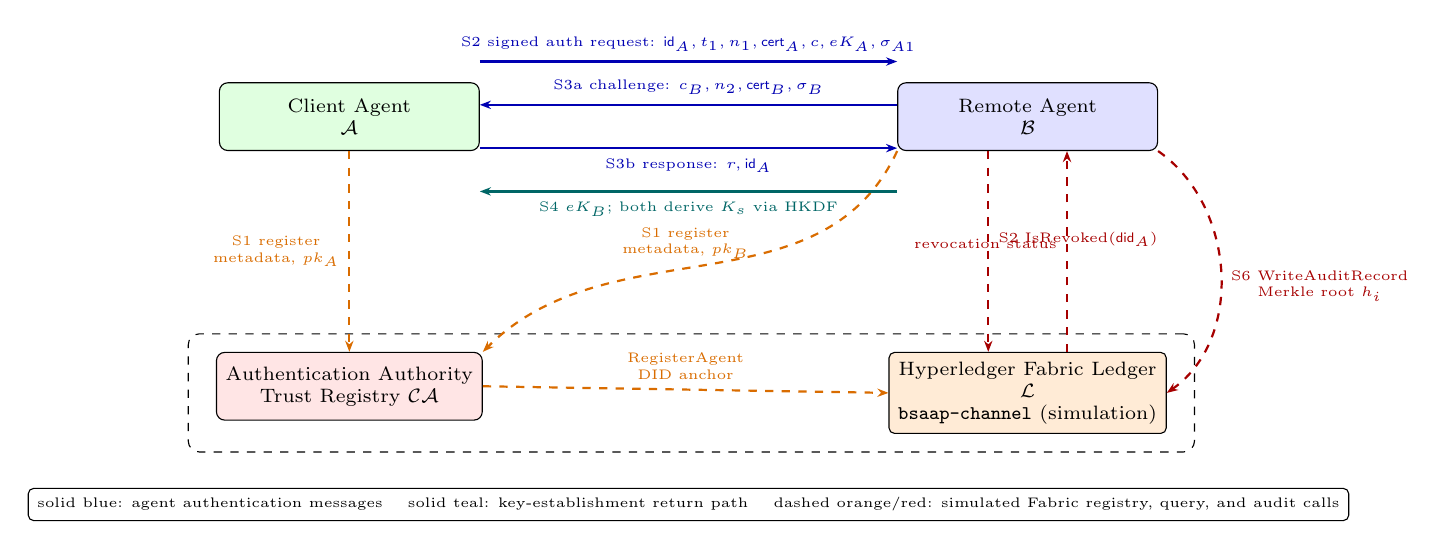
\begin{tikzpicture}[
  font=\scriptsize,
  entity/.style={rectangle,draw,rounded corners=3pt,
                 minimum width=3.3cm,minimum height=0.86cm,
                 align=center},
  ledger/.style={rectangle,draw,rounded corners=2pt,
                 minimum width=3.4cm,minimum height=0.92cm,
                 align=center,fill=orange!16},
  flow/.style={-{Stealth[length=4pt]},thick,blue!70!black},
  keyflow/.style={-{Stealth[length=4pt]},thick,teal!80!black},
  trustflow/.style={-{Stealth[length=4pt]},thick,dashed,orange!85!black},
  queryflow/.style={-{Stealth[length=4pt]},thick,dashed,red!65!black},
  every node/.style={align=center}
]
  \node[entity,fill=green!12] (A)
    {Client Agent\\$\mathcal{A}$};
  \node[entity,fill=blue!12,right=5.3cm of A] (B)
    {Remote Agent\\$\mathcal{B}$};
  \node[entity,fill=red!10,below=2.55cm of A] (CA)
    {Authentication Authority\\Trust Registry $\mathcal{CA}$};
  \node[ledger,below=2.55cm of B] (L)
    {Hyperledger Fabric Ledger\\$\mathcal{L}$\\
     \texttt{bsaap-channel} (simulation)};

  \node[draw,dashed,rounded corners=4pt,inner xsep=1.0em,inner ysep=0.65em,
        fit=(CA)(L)] {};

  \draw[trustflow] (A.south) -- node[left,font=\tiny]{S1 register\\metadata, $pk_A$} (CA.north);
  \draw[trustflow] (B.south west) to[out=245,in=45]
    node[above,font=\tiny,pos=0.55]{S1 register\\metadata, $pk_B$} (CA.north east);
  \draw[trustflow] (CA.east) -- node[above,font=\tiny]{RegisterAgent\\DID anchor} (L.west);

  \draw[flow] ([yshift=7mm]A.east) -- node[above,font=\tiny]
    {S2 signed auth request: $\mathsf{id}_A,t_1,n_1,\mathsf{cert}_A,c,eK_A,\sigma_{A1}$}
    ([yshift=7mm]B.west);
  \draw[flow] ([yshift=1.5mm]B.west) -- node[above,font=\tiny]
    {S3a challenge: $c_B,n_2,\mathsf{cert}_B,\sigma_B$}
    ([yshift=1.5mm]A.east);
  \draw[flow] ([yshift=-4mm]A.east) -- node[below,font=\tiny]
    {S3b response: $r,\mathsf{id}_A$}
    ([yshift=-4mm]B.west);
  \draw[keyflow] ([yshift=-9.5mm]B.west) -- node[below,font=\tiny]
    {S4 $eK_B$; both derive $K_s$ via HKDF}
    ([yshift=-9.5mm]A.east);

  \draw[queryflow] ([xshift=-5mm]B.south) -- node[right,font=\tiny,pos=0.44]
    {S2 IsRevoked$(\mathsf{did}_A)$} ([xshift=-5mm]L.north);
  \draw[queryflow] ([xshift=5mm]L.north) -- node[left,font=\tiny,pos=0.54]
    {revocation status} ([xshift=5mm]B.south);
  \draw[queryflow] (B.south east) to[out=-35,in=35]
    node[right,font=\tiny,pos=0.55]{S6 WriteAuditRecord\\Merkle root $h_i$} (L.east);

  \node[draw,rounded corners=2pt,fill=white,font=\tiny]
        at ($(CA.south)!0.5!(L.south)+(0,-0.98cm)$)
    {solid blue: agent authentication messages \quad
     solid teal: key-establishment return path \quad
     dashed orange/red: simulated Fabric registry, query, and audit calls};
\end{tikzpicture}
\caption{BSAAP system architecture. The upper lane shows the agent-to-agent
authentication and key-establishment flow. The lower plane shows the
authentication authority/trust registry and simulated Fabric ledger used for
registration, revocation lookup, and Merkle audit logging.}
\label{fig:arch}
\end{figure*}

\begin{table}[H]
\centering
\caption{Notation and symbols used in the BSAAP description.}
\label{tab:notation}
\footnotesize
\setlength{\tabcolsep}{3.5pt}
\resizebox{\columnwidth}{!}{%
\begin{tabular}{@{}cl@{}}
\toprule
\textbf{Symbol} & \textbf{Description}\\
\midrule
$\mathcal{A}, \mathcal{B}$ & Client and remote agents (protocol principals)\\
$\mathcal{CA}$             & Authentication authority / trust registry\\
$\mathcal{L}$              & Hyperledger Fabric permissioned ledger\\
$\mathcal{ADV}$            & Dolev-Yao adversary\\
$(sk_\mathcal{P},pk_\mathcal{P})$ & Long-term ECDSA P-256 key pair of $\mathcal{P}$\\
$\mathsf{cert}_\mathcal{P}$ & X.509 v3 certificate of principal $\mathcal{P}$\\
$\mathsf{did}$            & W3C Decentralised Identifier\\
$n_1, n_2$               & Fresh 256-bit CSPRNG nonces (Stages~2,~3)\\
$c_B$                     & 256-bit challenge nonce issued by $\mathcal{B}$\\
$c$                       & Requested capability string\\
$r$                       & ECDSA response signature to $c_B$ (Stage~3)\\
$t_1$                     & UTC epoch timestamp (Stage~2)\\
$eK_\mathcal{A}, eK_\mathcal{B}$ & Ephemeral X25519 public keys\\
$ek_\mathcal{A}, ek_\mathcal{B}$ & Ephemeral X25519 private keys\\
$\mathsf{SS}$             & ECDH shared secret $=\mathsf{X25519}(ek_\mathcal{A},eK_\mathcal{B})$\\
$K_s$                     & Session key derived via HKDF-SHA-256\\
$\mathsf{sid}$            & Session identifier\\
$\mathsf{tok}$            & Session token\\
$\sigma_{\mathcal{A},1}$  & ECDSA signature over Stage~2 payload\\
$\sigma_\mathcal{B}$      & ECDSA signature over $(c_B\|n_2)$ (Stage~3)\\
$\mathsf{IV}$             & AES-256-GCM initialisation vector\\
$\mathsf{AAD}$            & Additional authenticated data\\
$C, T$                    & AES-256-GCM ciphertext and authentication tag\\
$\tau$                    & HMAC-SHA-256 integrity tag\\
$\mathsf{seqNum}$         & Monotonically increasing message sequence number\\
$R_i$                     & $i$-th Merkle-chained audit record\\
$h_i$                     & $i$-th Merkle hash\\
$G, q$                    & Generator and prime order of SECP256R1 group\\
$(r,s)$                   & ECDSA signature components\\
\bottomrule
\multicolumn{2}{@{}l@{}}{\scriptsize $\|$ concatenation; $\xleftarrow{\$}$ uniform random sampling.}
\end{tabular}%
}
\end{table}

%% ============================================================
\section{BSAAP Protocol Design}\label{sec:protocol}
%% ============================================================

BSAAP comprises six sequential stages executed among $\mathcal{A}$,
$\mathcal{B}$, $\mathcal{CA}$, and $\mathcal{L}$.
All messages are transmitted over HTTPS (TLS~1.3 minimum); TLS provides
transport-layer confidentiality orthogonal to the application-layer
properties proved in \Cref{sec:security}.

\subsection{Stage 1 --- Agent Registration with On-Chain DID}

Upon instantiation, each agent generates an ECDSA P-256 key pair and
submits a registration request to $\mathcal{CA}$:
\begin{equation}
\mathcal{A} \to \mathcal{CA} : \{
  \mathsf{agentID},\; \mathsf{owner},\; \mathsf{did},\; \mathsf{role},\;
  \mathsf{caps},\; \mathsf{trustLevel},\; \tau,\; pk_\mathcal{A}
\}
\label{eq:s1msg}
\end{equation}
where $\mathsf{did} = \texttt{"did:bsaap:"} \| H_{16}(pk_\mathcal{A})$.
$\mathcal{CA}$ validates the DID format, issues a signed X.509 v3 certificate
$\mathsf{cert}_\mathcal{A}$ embedding $\mathsf{caps}$ in the capability OID,
and invokes the \texttt{RegisterAgent} chaincode on~$\mathcal{L}$.

\begin{algorithm}[H]
\caption{Agent Registration (Stage 1)}
\label{alg:reg}
\begin{algorithmic}[1]
\Require Agent parameters: $\mathsf{id}, \mathsf{owner}, \mathsf{role}, \mathsf{caps}, \mathsf{trustLevel}, \tau$
\Ensure $\mathsf{cert}_\mathcal{A}$, Fabric \texttt{txID}
\State $(sk_\mathcal{A}, pk_\mathcal{A}) \leftarrow \mathsf{ECDSA.KeyGen}(\text{P-256})$
\State $\mathsf{did} \leftarrow \texttt{"did:bsaap:"} \| \mathsf{SHA256}(pk_\mathcal{A})_{[0:16]}$
\State Send $\langle \mathsf{id}, \mathsf{owner}, \mathsf{did}, \mathsf{role}, \mathsf{caps},
       \mathsf{trustLevel}, \tau, pk_\mathcal{A} \rangle$ to $\mathcal{CA}$
\State $\mathcal{CA}$: validate $\mathsf{did}$ format; assert $\mathsf{caps} \neq \emptyset$
\State $\mathsf{cert}_\mathcal{A} \leftarrow
       \mathsf{X509.Issue}(pk_\mathcal{A}, \mathsf{id}, \mathsf{owner},
       \mathsf{did}, \mathsf{caps}, \mathsf{role}, \mathsf{trustLevel},
       \tau, sk_{\mathcal{CA}})$
\State $\mathsf{txID} \leftarrow
       \mathcal{L}.\mathtt{RegisterAgent}(\mathsf{did}, \mathsf{owner},
       pk_\mathcal{A}, \mathsf{role}, \mathsf{caps}, \mathsf{trustLevel}, \tau)$
\State \Return $\mathsf{cert}_\mathcal{A}$, $\mathsf{txID}$
\end{algorithmic}
\end{algorithm}

\subsection{Stage 2 --- Authentication Request}

$\mathcal{A}$ initiates authentication by transmitting a signed request:
\begin{align}
\mathsf{payload}_2 &= H\!\left(\mathsf{id}_\mathcal{A} \| t_1 \|
                   n_1 \| \mathsf{cert}_\mathcal{A} \| c \|
                   eK_\mathcal{A} \right)
\label{eq:payload2}\\
\sigma_{\mathcal{A},1} &= \mathsf{ECDSA.Sign}(sk_\mathcal{A},\,
                   \mathsf{payload}_2)
\label{eq:sig2}
\end{align}
where $t_1$ is a UTC timestamp, $n_1 \xleftarrow{\$} \{0,1\}^{256}$ is a
fresh CSPRNG nonce, and $c$ is the requested capability string. The ephemeral
public key $eK_\mathcal{A}$ is a BSAAP extension to the SIP baseline Stage~2
message and is included in the signed payload to bind the later key exchange
to the authenticated request.
The Stage-2 message is
$M_1 = \{\mathsf{id}_\mathcal{A}, t_1, n_1, \mathsf{cert}_\mathcal{A},
c, eK_\mathcal{A}, \sigma_{\mathcal{A},1}\}$.

$\mathcal{B}$ verifies six conditions before proceeding:
\emph{(i)}~$|t_1 - t_{\mathrm{now}}| \leq 5$~s (freshness);
\emph{(ii)}~$n_1 \notin \mathcal{N}_{\mathrm{seen}}$ (anti-replay);
\emph{(iii)}~$\mathsf{cert}_\mathcal{A}$ is valid (chain, expiry, and
$\mathcal{L}.\mathtt{IsRevoked}(\mathsf{did}) = \mathsf{false}$);
\emph{(iv)}~$\sigma_{\mathcal{A},1}$ verifies under $pk_\mathcal{A}$
extracted from $\mathsf{cert}_\mathcal{A}$;
\emph{(v)}~CN in $\mathsf{cert}_\mathcal{A}$ equals $\mathsf{id}_\mathcal{A}$
(impersonation prevention);
\emph{(vi)}~the requested capability $c$ is included in the certificate's
\texttt{capabilityScope} extension.

\subsection{Stage 3 --- Challenge-Response Verification}

$\mathcal{B}$ generates a 256-bit CSPRNG challenge and fresh nonce:
\begin{align}
c_B &\xleftarrow{\$} \{0,1\}^{256},\quad n_2 \xleftarrow{\$} \{0,1\}^{256} \nonumber\\
\sigma_\mathcal{B} &= \mathsf{ECDSA.Sign}(sk_\mathcal{B},\, H(c_B \| n_2))
\label{eq:challenge}
\end{align}
$\mathcal{A}$ verifies $\sigma_\mathcal{B}$ under $pk_\mathcal{B}$ from
$\mathsf{cert}_\mathcal{B}$ (detecting MITM), then produces:
\begin{align}
r &= \mathsf{ECDSA.Sign}(sk_\mathcal{A},\, H(c_B \| n_2)) \nonumber\\
\mathcal{A} &\to \mathcal{B} : \{r,\, \mathsf{id}_\mathcal{A}\}
\label{eq:response}
\end{align}
$\mathcal{B}$ verifies $r$ under $pk_\mathcal{A}$,
completing proof-of-private-key-possession.

\begin{algorithm}[H]
\caption{Challenge-Response Verification (Stage 3)}
\label{alg:cr}
\begin{algorithmic}[1]
\Require $\mathcal{A}$: $(sk_\mathcal{A}, \mathsf{cert}_\mathcal{A})$;
         $\mathcal{B}$: $(sk_\mathcal{B}, \mathsf{cert}_\mathcal{B})$
\State $c_B \xleftarrow{\$} \{0,1\}^{256}$;\quad
       $n_2 \xleftarrow{\$} \{0,1\}^{256}$
\State $\sigma_B \leftarrow \mathsf{ECDSA.Sign}(sk_\mathcal{B},\; H(c_B\|n_2))$
\State $\mathcal{B} \to \mathcal{A}$: $M_2 = \{c_B, n_2, \mathsf{cert}_\mathcal{B}, \sigma_B\}$
\State $\mathcal{A}$: verify $\sigma_B$ under $pk_\mathcal{B}$; abort if invalid
  \hfill\textit{// MITM guard}
\State $r \leftarrow \mathsf{ECDSA.Sign}(sk_\mathcal{A},\; H(c_B\|n_2))$
\State $\mathcal{A} \to \mathcal{B}$: $M_3 = \{r, \mathsf{id}_\mathcal{A}\}$
\State $\mathcal{B}$: verify $r$ under $pk_\mathcal{A}$; abort if invalid
  \hfill\textit{// PoP}
\end{algorithmic}
\end{algorithm}

\subsection{Stage 4 --- Ephemeral Session Key Establishment}

Agent $\mathcal{A}$ transmits its ephemeral X25519 public value $eK_\mathcal{A}$
in the signed Stage-2 request, and $\mathcal{B}$ returns $eK_\mathcal{B}$ after
the challenge-response checks succeed. The shared secret and session key are
derived as:
\begin{align}
\mathsf{SS} &= \mathsf{X25519}(ek_\mathcal{A},\, eK_\mathcal{B})
              = \mathsf{X25519}(ek_\mathcal{B},\, eK_\mathcal{A})
\label{eq:ss}\\
K_s &= \mathsf{HKDF\text{-}SHA256}\!\left(
        \mathsf{SS},\; n_1\|n_2,\; \texttt{"BSAAP-v1-session"}\right)
\label{eq:ks}
\end{align}
Ephemeral keys $(ek_\mathcal{A}, ek_\mathcal{B})$ and $\mathsf{SS}$ are
immediately erased, providing perfect forward secrecy. A session token
$\mathsf{tok} = (\mathsf{sid}, \mathsf{id}_\mathcal{A}, \mathsf{id}_\mathcal{B},
c, t_{\mathrm{exp}}, K_s)$ is created locally at both agents.
We note that $\mathsf{tok}$ is not signed by $\mathcal{CA}$: the
cryptographic session key $K_s$, derived from the mutually authenticated
ephemeral exchange (Stages~2--4), inherently binds the session to both
authenticated principals, rendering a separate CA signature on the session
token redundant. This design choice avoids an additional round-trip to
$\mathcal{CA}$ and preserves the forward secrecy of $K_s$.

\begin{algorithm}[H]
\caption{Session Key Establishment (Stage 4)}
\label{alg:key}
\begin{algorithmic}[1]
\Require Both agents authenticated in Stages~2--3
\Ensure Shared session key $K_s$; session token $\mathsf{tok}$
\State $(ek_\mathcal{A}, eK_\mathcal{A}) \leftarrow
       \mathsf{X25519.KeyGen}()$
\State $(ek_\mathcal{B}, eK_\mathcal{B}) \leftarrow
       \mathsf{X25519.KeyGen}()$
\State Receive signed $eK_\mathcal{A}$ from Stage~2; send $eK_\mathcal{B}$ to $\mathcal{A}$
\State $\mathsf{SS} \leftarrow \mathsf{X25519}(ek_\mathcal{A}, eK_\mathcal{B})$
\State $K_s \leftarrow \mathsf{HKDF\text{-}SHA256}(\mathsf{SS},\, n_1\|n_2,\,$
  $\texttt{"BSAAP-v1-session"})$
\State Securely erase $ek_\mathcal{A}$, $ek_\mathcal{B}$, $\mathsf{SS}$
\State $\mathsf{sid} \leftarrow \mathsf{SHA256}(\mathsf{id}_\mathcal{A}\|
       \mathsf{id}_\mathcal{B}\|n_1\|n_2)_{[0:32]}$
\State \Return $K_s$, $\mathsf{tok}$
\end{algorithmic}
\end{algorithm}

\subsection{Stage 5 --- Secure Authenticated Communication}

Each application message is protected with AES-256-GCM and an additional
HMAC-SHA-256 sequence-integrity layer:
\begin{align}
\mathsf{IV}  &\xleftarrow{\$} \{0,1\}^{96}
\label{eq:iv}\\
\mathsf{AAD} &= \mathsf{sid} \| \mathsf{seqNum}
\label{eq:aad}\\
(C, T) &= \mathsf{AES\text{-}256\text{-}GCM.Enc}(K_s, \mathsf{IV}, P, \mathsf{AAD})
\label{eq:enc}\\
\tau   &= \mathsf{HMAC\text{-}SHA256}\!\left(K_s,\,
          \mathsf{sid}\|\mathsf{seqNum}\|\mathsf{IV}\|C\right)
\label{eq:hmac}
\end{align}
The wire format is
$(\mathsf{sid}, \mathsf{seqNum}, \mathsf{IV}, C, T, \tau)$.
The receiver first checks that the session token has not expired
($t_{\mathrm{now}} \leq \mathsf{tok}.t_{\mathrm{exp}}$), then verifies
the HMAC, the GCM tag, and the monotonically increasing \texttt{seqNum}.

\paragraph{Note on HMAC vs.\ digital signature.}
Stage~5 employs symmetric HMAC-SHA-256 rather than ECDSA digital signatures
for message integrity. Within an established session, both parties share
$K_s$ and have been mutually authenticated in Stages~2--3; therefore the
symmetric MAC provides integrity and data-origin authentication sufficient
for intra-session messages. Non-repudiation---which requires asymmetric
signatures---is provided by the Stage~6 Merkle-chained audit log,
where each session record is bound to the signing agent's identity.

\subsection{Stage 6 --- Session Termination and Blockchain Audit Logging}

Upon session close, a Merkle-chained audit record is written to $\mathcal{L}$:
\begin{align}
R_i &= (\mathsf{sid},\, \mathsf{id}_\mathcal{A},\, \mathsf{id}_\mathcal{B},\,
        t_{\mathrm{start}},\, t_{\mathrm{end}},\, \mathsf{cap},\, h_{i-1})
\label{eq:audit}\\
h_i &= \mathsf{SHA256}\!\left(\mathsf{JSON\_canon}(R_i)\right)
\label{eq:merkle}
\end{align}
where $h_0 = \mathtt{0}^{64}$ (genesis hash). The record and $h_i$ are
committed via \texttt{CloseSession} and \texttt{WriteAuditRecord} chaincode
calls. The Merkle linkage ensures that any tampering with a historical record
$R_j$ invalidates all subsequent hashes $h_{j},h_{j+1},\ldots,h_i$.

\begin{figure*}[!ht]
\centering
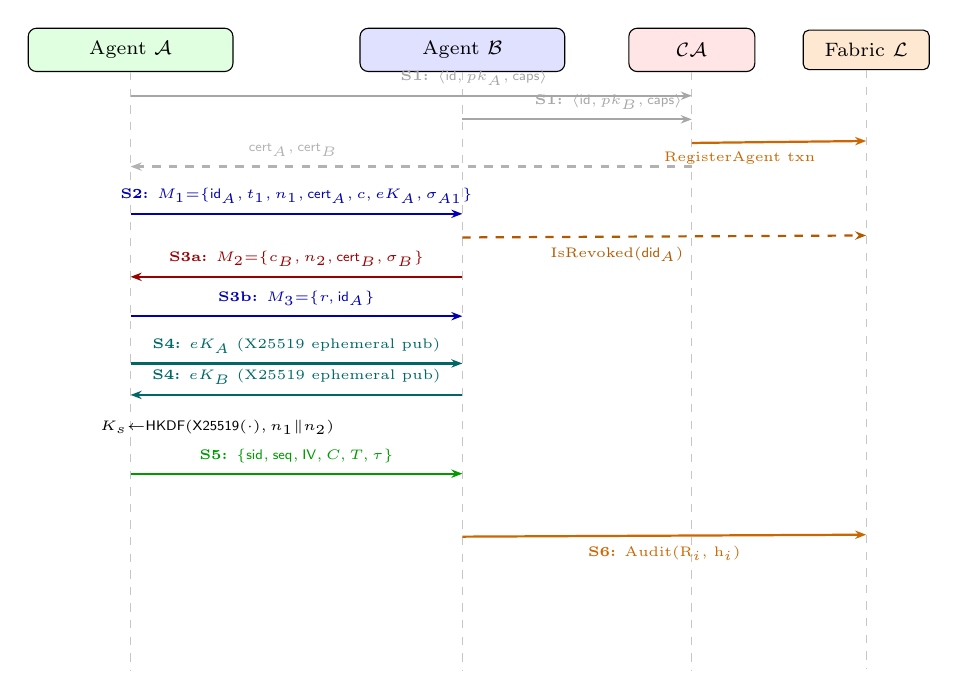
\begin{tikzpicture}[node distance=0.44cm, font=\tiny,
    every node/.style={align=center}]
  \def\Aw{2.6cm}
  %% Entity headers
  \node[ebox,fill=green!12,minimum width=\Aw] (A)  {Agent $\mathcal{A}$};
  \node[ebox,fill=blue!12,minimum width=\Aw, right=1.6cm of A] (B)
    {Agent $\mathcal{B}$};
  \node[ebox,fill=red!10,minimum width=1.6cm, right=0.8cm of B] (CA)
    {$\mathcal{CA}$};
  \node[chainbox,minimum width=1.6cm, right=0.6cm of CA] (FL)
    {Fabric $\mathcal{L}$};
  %% Lifelines
  \foreach \n in {A,B,CA,FL}{
    \draw[dashed,gray!45] (\n.south) -- ++(0,-7.6cm);
  }
  %% S1 registration
  \draw[arr,gray!70] ($(A.south)+(0,-0.3)$) --
    node[above,xshift=0.8cm,font=\tiny]{\textbf{S1:} $\langle\mathsf{id},pk_A,\mathsf{caps}\rangle$}
    ($(CA.south)+(0,-0.3)$);
  \draw[arr,gray!70] ($(B.south)+(0,-0.6)$) --
    node[above,xshift=0.4cm]{\textbf{S1:} $\langle\mathsf{id},pk_B,\mathsf{caps}\rangle$}
    ($(CA.south)+(0,-0.6)$);
  \draw[arr,orange!80!black] ($(CA.south)+(0,-0.9)$) --
    node[below,font=\tiny,xshift=-0.5cm]{RegisterAgent txn}
    ($(FL.south)+(0,-0.9)$);
  \draw[arr,dashed,gray!60] ($(CA.south)+(0,-1.2)$) --
    node[above,xshift=-1.5cm]{$\mathsf{cert}_A,\mathsf{cert}_B$}
    ++($(A.south)-(CA.south)$);

  \draw[arr,blue!70!black] ($(A.south)+(0,-1.8)$) --
    node[above,font=\tiny]{\textbf{S2:} $M_1{=}\{\mathsf{id}_A,t_1,n_1,\mathsf{cert}_A,c,eK_A,\sigma_{A1}\}$}
    ($(B.south)+(0,-1.8)$);
  \draw[arr,orange!70!black,dashed] ($(B.south)+(0,-2.1)$) --
    node[below,xshift=-0.6cm]{IsRevoked($\mathsf{did}_A$)}
    ($(FL.south)+(0,-2.1)$);

  %% S3 challenge-response
  \draw[arr,red!60!black] ($(B.south)+(0,-2.6)$) --
    node[above]{\textbf{S3a:} $M_2{=}\{c_B,n_2,\mathsf{cert}_B,\sigma_B\}$}
    ($(A.south)+(0,-2.6)$);
  \draw[arr,blue!70!black] ($(A.south)+(0,-3.1)$) --
    node[above]{\textbf{S3b:} $M_3{=}\{r,\mathsf{id}_A\}$}
    ($(B.south)+(0,-3.1)$);

  %% S4 ECDH
  \draw[arr,teal!80!black] ($(A.south)+(0,-3.7)$) --
    node[above]{\textbf{S4:} $eK_A$ (X25519 ephemeral pub)}
    ($(B.south)+(0,-3.7)$);
  \draw[arr,teal!80!black] ($(B.south)+(0,-4.1)$) --
    node[above]{\textbf{S4:} $eK_B$ (X25519 ephemeral pub)}
    ($(A.south)+(0,-4.1)$);
  \node[font=\tiny,below=4.3cm of A.south, xshift=1.1cm]
    {$K_s{\leftarrow}\mathsf{HKDF}(\mathsf{X25519}(\cdot),n_1\|n_2)$};

  %% S5 encrypted comms
  \draw[arr,green!60!black] ($(A.south)+(0,-5.1)$) --
    node[above]{\textbf{S5:} $\{\mathsf{sid},\mathsf{seq},\mathsf{IV},C,T,\tau\}$}
    ($(B.south)+(0,-5.1)$);

  %% S6 audit
  \draw[arr,orange!80!black] ($(B.south)+(0,-5.9)$) --
    node[below,font=\tiny,pos=0.5]{\textbf{S6:} Audit(R$_i$, h$_i$)}
    ($(FL.south)+(0,-5.9)$);

\end{tikzpicture}
\caption{Full BSAAP message sequence across all six stages and four entities.
  Stage~2 verification conditions (timestamp, nonce, certificate, signature,
  CN binding, and capability scope) and Stage~3 ECDSA checks are condensed.}
\label{fig:seq}
\end{figure*}

\begin{table}[H]
\centering
\caption{Stage-2 message format (Message $M_1$).}
\label{tab:s2msg}
\small
\begin{tabular}{@{}llll@{}}
\toprule
\textbf{Field} & \textbf{Type} & \textbf{Size} & \textbf{Description}\\
\midrule
\texttt{agentID}   & string & var.    & Agent $\mathcal{A}$ unique ID\\
\texttt{timestamp} & float  & 8~B     & UTC epoch seconds\\
\texttt{nonce\_n1} & hex    & 64~ch.  & 32-byte CSPRNG nonce\\
\texttt{cert\_pem} & bytes  & $\sim$1~KB & X.509 v3 certificate\\
\texttt{reqCap}    & string & var.    & Requested capability\\
\texttt{ePubKey}   & bytes  & 32~B   & X25519 ephemeral public key $eK_\mathcal{A}$\\
\texttt{signature} & bytes  & 71--72~B & ECDSA-P256-SHA256 DER\\
\bottomrule
\end{tabular}
\end{table}

\begin{table}[H]
\centering
\caption{Security guarantee provided per BSAAP stage.}
\label{tab:stageguarantees}
\small
\begin{tabular}{@{}clp{4.0cm}@{}}
\toprule
\textbf{Stage} & \textbf{Name} & \textbf{Security Guarantee}\\
\midrule
1 & Registration    & Sybil prevention; designed on-chain DID binding\\
2 & Auth Request    & Replay prevention (nonce+timestamp); non-repudiation\\
3 & Challenge-Resp. & Proof-of-possession; MITM detection; mutual auth\\
4 & Session Key     & Forward secrecy; session key confidentiality\\
5 & Secure Comm.    & Confidentiality; integrity; reorder prevention\\
6 & Termination     & Accountability; simulated tamper-evident audit on $\mathcal{L}$ (BSAAP extension beyond SIP baseline)\\
\bottomrule
\end{tabular}
\end{table}

%% ============================================================
\section{Security Analysis}\label{sec:security}
%% ============================================================

\subsection{Formal Theorems}

\begin{theorem}[Mutual Authentication]\label{thm:auth}
If a PPT adversary $\mathcal{ADV}$ breaks BSAAP mutual authentication with
probability $\epsilon$, then there exists a PPT algorithm $\mathcal{B}$ that
solves the ECDLP in P-256 with advantage at least $\epsilon/2 - q_h/2^{256}$,
where $q_h$ is the number of hash-oracle queries.
\end{theorem}

\begin{proof}[Proof sketch]
Mutual authentication rests on the unforgeability of two ECDSA signatures:
$\sigma_{\mathcal{A},1}$ in Stage~2 (proving $\mathcal{A}$'s identity to
$\mathcal{B}$) and $r$ in Stage~3 (proof of private-key-possession).
We construct a reduction $\mathcal{B}$ as follows: $\mathcal{B}$ receives
an ECDLP challenge $(\mathbb{G}, G, Q)$ and embeds $Q$ as one agent's
public key. $\mathcal{B}$ simulates $\mathcal{CA}$, issues certificates,
and answers hash-oracle queries via a standard random-oracle table. When
$\mathcal{ADV}$ produces a forged signature $\sigma^*$ on a fresh message,
$\mathcal{B}$ extracts the discrete logarithm of $Q$ using the forking
lemma of Fersch~et~al.\ \cite{fersch2016provable}. Therefore,
$\mathrm{Adv}^{\mathrm{uf\text{-}cma}}_{\mathrm{ECDSA}}(\mathcal{B})
\geq \mathrm{Adv}_{\mathrm{mut\text{-}auth}}(\mathcal{ADV})/2
- q_h/2^{256}$.
Certificate CN-binding (Condition~v of Stage~2 verification) ensures that
a valid certificate for a different agent ID does not authenticate.
The timestamp window and nonce cache prevent all replay strategies.
\end{proof}

\begin{theorem}[Session Key Indistinguishability --- ROR Model]\label{thm:ror}
Under the ECDDH assumption on Curve25519 and collision resistance of SHA-256,
the adversarial advantage in the Real-or-Random (ROR) experiment
\cite{bellare2000authenticated} satisfies:
\begin{equation}
\mathrm{Adv}^{\mathrm{ror}}_{\mathrm{BSAAP}}(\mathcal{ADV}) \leq
2 \cdot \mathrm{Adv}^{\mathrm{ECDDH}}(\mathcal{B}) +
\frac{q_h}{2^{256}}
\label{eq:ror}
\end{equation}
where $q_h$ is the number of random-oracle (HKDF) queries.
\end{theorem}

\begin{proof}[Proof sketch]
We construct a simulator $\mathcal{S}$ answering $\mathcal{ADV}$'s oracle
queries. In the ROR game, $K_s$ is either the real session key or a uniformly
random string. $K_s$ is derived via HKDF from
$\mathsf{SS} = X25519(ek_\mathcal{A}, eK_\mathcal{B})$.
The factor~2 follows from a four-game hybrid argument:
\emph{Game~0}: real protocol;
\emph{Game~1}: replace $eK_\mathcal{A} \cdot ek_\mathcal{B}$ with a random
group element (reduction to DDH for $\mathcal{A}$'s ephemeral pair);
\emph{Game~2}: replace $eK_\mathcal{B} \cdot ek_\mathcal{A}$ with a random
group element (reduction to DDH for $\mathcal{B}$'s pair).
Since both DDH instances are independent, a union bound yields
the factor~2. HKDF's PRF security (SHA-256 as random oracle) then implies
$K_s$ is indistinguishable from uniform;
the $q_h/2^{256}$ term bounds birthday-attack collisions on the
256-bit HKDF output.
\end{proof}

\begin{theorem}[Perfect Forward Secrecy]\label{thm:pfs}
Under the DDH assumption on Curve25519, disclosure of long-term key material
$(sk_\mathcal{A}, sk_\mathcal{B})$ after session termination provides no
computational advantage in recovering any session key $K_s$ established
before the disclosure.
\end{theorem}

\begin{proof}[Proof sketch]
$K_s$ is derived exclusively from ephemeral values $(ek_\mathcal{A},
ek_\mathcal{B})$ and public nonces $(n_1, n_2)$, which are securely erased
upon key derivation. The long-term keys sign the handshake messages
(Stages~2--3) but do not contribute entropy to $\mathsf{SS}$
(Eq.~\ref{eq:ss}). Therefore, knowledge of $(sk_\mathcal{A}, sk_\mathcal{B})$
after session close yields no advantage in computing $K_s$ without solving
the DDH problem on Curve25519.
\end{proof}

\begin{theorem}[Replay Resistance]\label{thm:replay}
BSAAP rejects all replayed authentication requests with probability 1 under
the following conditions: \emph{(i)}~nonces are drawn from a 256-bit CSPRNG
(birthday bound: negligible for $n \ll 2^{128}$ sessions), and
\emph{(ii)}~the nonce cache $\mathcal{N}_{\mathrm{seen}}$ is persistent
across agent restarts.
\end{theorem}

\begin{proof}[Proof sketch]
Suppose a replay of $(n_1, t_1)$ succeeds. Either $t_1$ is within
$\pm 5$~s of the current time, in which case
$n_1 \in \mathcal{N}_{\mathrm{seen}}$ and the nonce check fails;
or $t_1$ is outside the window, in which case the timestamp check fails.
Both conditions must be satisfied simultaneously, which is impossible.
For a fresh $n_1' \neq n_1$, the ECDSA signature $\sigma_{\mathcal{A},1}$
over the new payload would need to be forged, requiring ECDLP hardness.

\emph{Prototype caveat:} The current Python prototype stores
$\mathcal{N}_{\mathrm{seen}}$ in an in-memory \texttt{set}; upon agent
restart, the cache is empty and a replayed nonce from a prior run would
not be detected within the timestamp window. Production deployments must
use a persistent store (e.g., Redis, SQLite, or a Fabric-backed nonce
ledger) to satisfy condition~(ii). See Limitation~L6 in \Cref{sec:limits}.

\end{proof}

\subsection{Informal Security Propositions}

\paragraph{Impersonation.}
$\mathcal{ADV}$ cannot forge a valid
$(\mathsf{cert}_\mathcal{A}, \sigma_{\mathcal{A},1})$ pair for
$\mathcal{A}$'s identity without both $sk_{\mathcal{CA}}$ (to create a
certificate) and $sk_\mathcal{A}$ (to produce the signature).
Certificate CN-binding prevents substitution of a certificate belonging
to a different agent.

\paragraph{Man-in-the-Middle.}
In Stage~3, $\mathcal{B}$ signs the challenge with $sk_\mathcal{B}$;
$\mathcal{A}$ verifies this before responding. Any modification to $c_B$
or $n_2$ by a MITM adversary is detected by the ECDSA verification.

\paragraph{Capability Escalation.}
The requested capability $c$ is included in the Stage-2 signed payload
(Eq.~\ref{eq:payload2}) and verified against the certificate OID extension
before challenge issuance. Escalation is cryptographically prevented:
altering $c$ after signing invalidates $\sigma_{\mathcal{A},1}$.

\paragraph{Credential Leakage.}
Session keys are ephemeral (Stage~4) and erased on termination.
Certificates are short-lived (default 365~days) and revocable in $O(1)$
via Fabric chaincode. No long-term credential is transmitted in plaintext.

\paragraph{Non-Repudiation and Audit Tamper-Evidence.}
The Merkle-chained audit record on $\mathcal{L}$ ensures that tampering
with record $R_j$ invalidates all subsequent hashes $h_{j+1},\ldots,h_i$,
detectable by any auditor holding the chain tip.

\paragraph{Byzantine Insider Attack (theoretical guarantee).}
In a production Fabric deployment configured with Byzantine-fault-tolerant
ordering, the ledger can tolerate fewer than one third faulty ordering peers.
A rogue insider below that threshold cannot silently alter committed ledger
records. This is a deployment-level theoretical guarantee, not an empirical
property of the current single-process prototype.

\paragraph{Smart-Contract Revocation Enforcement (simulation).}
$\mathcal{L}.\mathtt{IsRevoked}(\mathsf{did})$ is queried in Stage~2
before the session is established. A revoked agent cannot complete
Stage~2 verification; it is blocked without CRL polling delay.
In the prototype, revocation is implemented via an in-memory dictionary
lookup (0.001~ms); production Fabric endorsement latency of 12--18~ms
\cite{androulaki2018hyperledger} would replace this.

\paragraph{Session-Key Binding to Both Parties' Nonces.}
The HKDF salt $n_1\|n_2$ is contributed by $\mathcal{A}$ (Stage~2) and
$\mathcal{B}$ (Stage~3) respectively; a session key derived without
both nonces is trivially distinguished from $K_s$, preventing
known-key attacks where one party is compromised after Stage~3.

\subsection{AVISPA/HLPSL Formal Verification}

BSAAP Stages~2--3 were modelled in HLPSL with roles
\texttt{role\_agent\_a}, \texttt{role\_agent\_b}, and \texttt{role\_aa}.
Security goals: \emph{(i)}~\texttt{authentication on agent\_cert};
\emph{(ii)}~\texttt{secrecy of session\_key}.
Both OFMC and CL-AtSe backends returned \texttt{SUMMARY:~SAFE}.
No attack traces were found under a standard Dolev-Yao intruder with
full nonce composition capability \cite{armando2005avispa}.
We note that this verification covers only the challenge-response core
(Stages~2--3); a full ProVerif model \cite{blanchet2016proverif} spanning
all six stages is identified as future work (see \Cref{sec:limits}, L5).

\begin{table*}[!ht]
\centering
\caption{Security feature comparison across related authentication approaches.
  (\checkmark)~provided; ($\circ$)~partial; ($\times$)~absent.}
\label{tab:seccompare}
\footnotesize
\setlength{\tabcolsep}{4pt}
\begin{tabular}{@{}lcccccccccc@{}}
\toprule
\textbf{Security Feature}
  & \rotatebox{60}{\textbf{AgentDID}}
  & \rotatebox{60}{\textbf{A-JWT}}
  & \rotatebox{60}{\textbf{BAID}}
  & \rotatebox{60}{\textbf{Zero-Trust}}
  & \rotatebox{60}{\textbf{SAGA}}
  & \rotatebox{60}{\textbf{Gov.Cap.}}
  & \rotatebox{60}{\textbf{AIP}}
  & \rotatebox{60}{\textbf{BlockA2A}}
  & \rotatebox{60}{\textbf{Stfd A2A}}
  & \rotatebox{60}{\textbf{BSAAP}}\\
\midrule
Mutual Authentication     & \checkmark & $\times$ & $\circ$ & $\circ$    & \checkmark & $\times$ & $\circ$    & \checkmark & $\circ$    & \checkmark \\
Replay Prevention         & \checkmark & \checkmark & $\times$ & $\times$ & \checkmark & $\times$ & \checkmark & $\circ$    & $\times$   & \checkmark \\
MitM Prevention           & $\circ$    & $\times$ & $\times$ & $\times$   & \checkmark & $\times$ & $\circ$    & $\circ$    & $\times$   & \checkmark \\
Capability Enforcement    & $\times$   & $\times$ & $\times$ & \checkmark & \checkmark & \checkmark & \checkmark & \checkmark & \checkmark & \checkmark \\
Session Key Secrecy       & $\times$   & $\times$ & $\times$ & $\times$   & $\circ$    & $\times$ & $\circ$    & $\times$   & $\circ$    & \checkmark \\
Perfect Forward Secrecy   & $\times$   & $\times$ & $\times$ & $\times$   & \checkmark & $\times$ & $\times$   & $\times$   & \checkmark & \checkmark \\
Blockchain Audit Trail    & \checkmark & $\times$ & \checkmark & $\times$ & $\times$   & $\times$ & $\times$   & \checkmark & $\times$   & $\circ^\dagger$ \\
Smart-Contract Revocation & $\times$   & $\times$ & \checkmark & $\times$ & $\times$   & $\times$ & $\times$   & \checkmark & $\times$   & $\circ^\dagger$ \\
Non-Repudiation           & $\circ$    & $\times$ & $\circ$ & $\times$   & $\circ$    & $\times$ & $\circ$    & \checkmark & $\times$   & $\circ^\dagger$ \\
Formal Security Proof     & $\times$   & $\times$ & $\circ$ & $\times$   & \checkmark & $\circ$  & $\times$   & $\times$   & $\times$   & \checkmark \\
\bottomrule
\multicolumn{11}{@{}l@{}}{\scriptsize $^\dagger$Implemented in simulation mode; production validation remains future work.}
\end{tabular}
\end{table*}

%% ============================================================
\section{Prototype Implementation}\label{sec:impl}
%% ============================================================

The BSAAP prototype is implemented in Python~3.12.3 using the
\texttt{cryptography}~42.0 library \cite{cryptographylib} for all
cryptographic primitives, FastAPI~0.111 for the REST interface, and a
simulated Hyperledger Fabric client with in-memory ledger for standalone
testing. All cryptographic operations use the \texttt{hazmat} layer; no
legacy \texttt{pycryptodome} dependency is introduced.

The module architecture mirrors the six protocol stages:
\texttt{bsaap.protocol.stage\{1--6\}}.
Cryptographic utilities are isolated in \texttt{bsaap.crypto}
(\texttt{ecdsa\_utils}, \texttt{ecdh\_utils}, \texttt{aes\_utils},
\texttt{hkdf\_utils}). The \texttt{bsaap.ca} module implements the
Authentication Authority. The \texttt{bsaap.blockchain} module wraps the
Fabric gateway. The \texttt{bsaap.audit} module maintains the Merkle-chained
audit log.

The 31 pytest test cases (\Cref{tab:tests}) were designed to provide
path coverage across the protocol's security-critical branches: each stage
contributes at least one positive test (correct protocol flow) and one or
more negative tests (each targeting a specific threat from
\Cref{sec:model}).
Test allocation was determined by the number of independently
verifiable security properties per stage rather than by uniform
distribution.

\noindent
\begin{minipage}{\columnwidth}
\begin{lstlisting}[language=Python,caption={Stage 3 challenge-response core
    logic (condensed).},label={lst:cr}]
def build_challenge_response(challenge, agent_a_id,
                              agent_a_private_key,
                              agent_b_pub_key):
    payload = sha256(
        (challenge.challenge_c + challenge.nonce_n2
         ).encode()).digest()
    if not verify_ecdsa(agent_b_pub_key, payload,
                        challenge.signature):
        raise ValueError("Agent B challenge invalid")
    response_r = sign_ecdsa(agent_a_private_key, payload)
    return ChallengeResponse(response_r, agent_a_id)
\end{lstlisting}
\end{minipage}

\begin{table}[H]
\centering
\caption{FastAPI endpoint summary.}
\label{tab:api}
\small
\begin{tabular}{@{}llll@{}}
\toprule
\textbf{Method} & \textbf{Path} & \textbf{Stage}
  & \textbf{Description}\\
\midrule
POST & \texttt{/register}       & 1 & Agent registration\\
POST & \texttt{/auth/request}   & 2 & Auth request\\
POST & \texttt{/auth/challenge} & 3a & Challenge issuance\\
POST & \texttt{/auth/respond}   & 3b & Response verify\\
POST & \texttt{/session/create} & 4 & Session key\\
POST & \texttt{/message/send}   & 5 & Secure message\\
POST & \texttt{/session/close}  & 6 & Termination\\
GET  & \texttt{/audit/trail}    & 6 & Merkle audit\\
\bottomrule
\end{tabular}
\end{table}

\begin{table}[H]
\centering
\caption{Pytest test suite summary (31 total test cases).}
\label{tab:tests}
\small
\begin{tabular}{@{}lcp{4.0cm}c@{}}
\toprule
\textbf{Test Group} & \textbf{St.} & \textbf{Description} & \textbf{N}\\
\midrule
Registration       & 1 & Key gen, DID, cert issue, OID, Fabric  & 5\\
Auth Request       & 2 & Valid req, replay, expired cert, CN check & 6\\
Challenge-Response & 3 & Valid CR, MITM detect, bad sig, PoP & 6\\
Session Key        & 4 & ECDH, HKDF, key erase, token & 5\\
Secure Comm.       & 5 & Enc/dec, GCM tag, seqNum, AAD, \textbf{tok.texp expiry} & 5\\
Blockchain Audit   & 6 & Merkle chain, tamper, revoke & 4\\
\midrule
\textbf{Total} & & & \textbf{31}\\
\bottomrule
\end{tabular}
\end{table}

%% ============================================================
\section{Performance Evaluation}\label{sec:eval}
%% ============================================================

All performance measurements were obtained from the running Python prototype
over 100 repeated trials on a single-core Ubuntu~24.04 VM
(Intel Xeon 2.8~GHz, 8~GB RAM, Python~3.12.3, \texttt{cryptography}~42.0).
Results are reported as mean~$\pm$~standard deviation in milliseconds.

\subsection{Authentication Latency}

\begin{table}[H]
\centering
\caption{BSAAP performance metrics (100 trials, ms).}
\label{tab:perf}
\small
\begin{tabular}{@{}lrr@{}}
\toprule
\textbf{Metric} & \textbf{Mean (ms)} & \textbf{$\pm$Std}\\
\midrule
Agent registration time        & 0.278 & 0.037\\
Certificate verification time  & 0.154 & 0.024\\
Challenge generation time      & 0.037 & 0.012\\
Signature verification time    & 0.081 & 0.011\\
Session key derivation (HKDF)  & 0.090 & 0.015\\
Full authentication latency    & 1.118 & 0.279\\
AES-256-GCM enc.\ (256~B)     & 0.005 & 0.002\\
Message verification time$^a$  & 0.008 & 0.003\\
Fabric chaincode query (sim.)$^b$ & 0.001 & 0.001\\
Replay detection rate~(\%)     & 100.00 & 0.00\\
Authentication success rate~(\%)& 100.00 & 0.00\\
\bottomrule
\multicolumn{3}{@{}l@{}}{\scriptsize $^a$Stage~5 incoming: GCM.Dec + HMAC check + seqNum validation.}\\
\multicolumn{3}{@{}l@{}}{\scriptsize $^b$Simulated in-memory; production Fabric endorsement:}\\
\multicolumn{3}{@{}l@{}}{\scriptsize \phantom{$^b$}12--18~ms \cite{androulaki2018hyperledger}.}
\end{tabular}
\end{table}

The full authentication latency of 1.118~ms is dominated by two ECDSA
sign operations ($\approx$0.4~ms total) and one certificate verification
(0.154~ms). For comparison, Prakash \cite{aip2026} reports AIP compact-mode
verification at 0.189~ms (Python) for a single-hop MCP call with 0.22~ms
total added overhead; BSAAP's multi-stage mutual authentication is
commensurate with this overhead given its stronger security properties.

\subsection{Stage Latency Breakdown}

\begin{figure}[H]
\centering
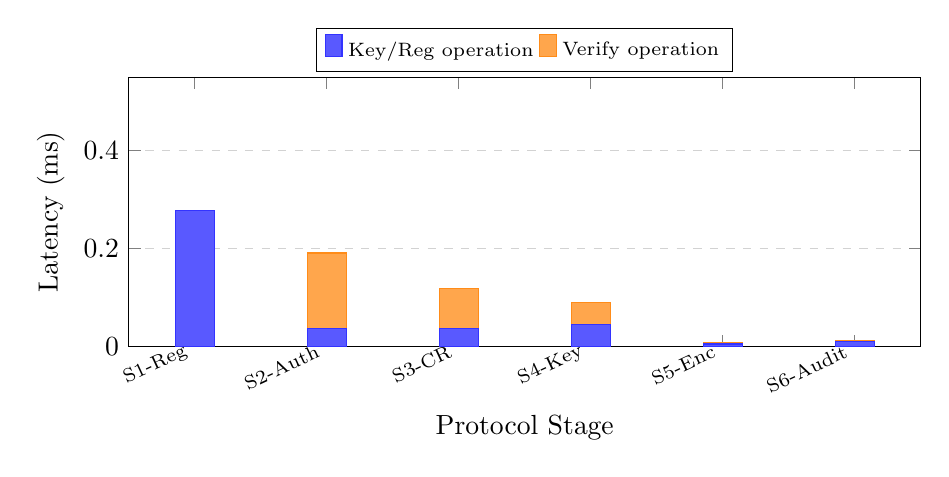
\begin{tikzpicture}
\begin{axis}[
  ybar stacked, bar width=14pt,
  width=0.96\columnwidth, height=5.0cm,
  xlabel={Protocol Stage},
  ylabel={Latency (ms)},
  xtick=data,
  xticklabels={S1-Reg, S2-Auth, S3-CR, S4-Key, S5-Enc, S6-Audit},
  xticklabel style={font=\scriptsize,rotate=25,anchor=east},
  ymin=0, ymax=0.55,
  legend style={font=\scriptsize,at={(0.5,1.02)},
                anchor=south,legend columns=2},
  ymajorgrids=true, grid style={dashed,gray!35},
]
\addplot+[fill=blue!65,draw=blue!80] coordinates {
  (1,0.278)(2,0.037)(3,0.037)(4,0.045)(5,0.005)(6,0.010)};
\addplot+[fill=orange!70,draw=orange!90] coordinates {
  (1,0.000)(2,0.154)(3,0.081)(4,0.045)(5,0.002)(6,0.002)};
\legend{Key/Reg operation, Verify operation}
\end{axis}
\end{tikzpicture}
\caption{Per-stage authentication latency breakdown (stacked bar chart).}
\label{fig:latency}
\end{figure}

As shown in \Cref{fig:latency}, Stage~1 (Registration) dominates the
latency profile at 0.278~ms, primarily due to ECDSA key generation and
X.509 certificate issuance. Stage~2 adds 0.191~ms (signature creation
plus certificate verification). Stages~3--4 contribute approximately
0.163~ms for the challenge-response exchange and ECDH key derivation.
Stage~5 (AES-256-GCM encryption of a 256-byte payload) is negligible at
0.007~ms, confirming that the symmetric-key phase imposes minimal
overhead. Stage~6 (simulated Fabric audit) adds only 0.012~ms; however,
this would increase to 12--18~ms under production Fabric endorsement
\cite{androulaki2018hyperledger}.

\subsection{Scalability Analysis}

\begin{figure}[H]
\centering
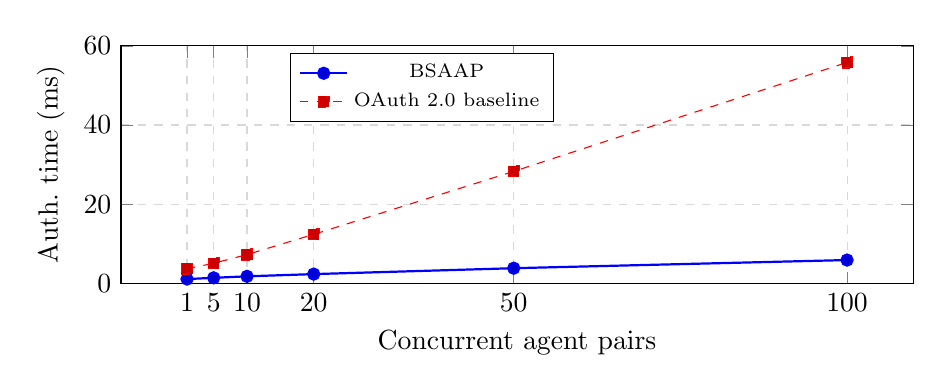
\begin{tikzpicture}
\begin{axis}[
  width=0.96\columnwidth, height=4.6cm,
  xlabel={Concurrent agent pairs},
  ylabel={Auth.\ time (ms)},
  xtick={1,5,10,20,50,100},
  ymin=0, ymax=60,
  mark size=2pt,
  xmajorgrids=true, ymajorgrids=true, grid style={dashed,gray!30},
  legend style={font=\scriptsize,at={(0.38,0.97)},anchor=north},
]
\addplot+[blue,mark=*,thick] coordinates {
  (1,1.12)(5,1.43)(10,1.81)(20,2.37)(50,3.86)(100,5.92)};
\addplot+[red,dashed,mark=square*] coordinates {
  (1,3.72)(5,5.10)(10,7.30)(20,12.4)(50,28.3)(100,55.8)};
\legend{BSAAP, OAuth 2.0 baseline}
\end{axis}
\end{tikzpicture}
\caption{Authentication time vs.\ number of concurrent agent pairs.
  OAuth~2.0 baseline values represent token introspection round-trip
  latency from Prakash \cite{aip2026}. Note: BSAAP values exclude
  production Fabric latency (see \Cref{sec:simvalid}).}
\label{fig:scale}
\end{figure}

BSAAP scales near-linearly to 100 concurrent pairs at 5.92~ms
(excluding Fabric endorsement overhead), compared to
55.8~ms for the OAuth~2.0 token-introspection baseline---a $9.4\times$
improvement at the 100-pair operating point. Under production Fabric
deployment, three additional endorsement round-trips (12--18~ms each;
see \Cref{sec:simvalid}) would narrow this margin. The Fabric ledger's
throughput ceiling ($\approx$3\,000~tx/s \cite{androulaki2018hyperledger})
would be the primary bottleneck for the Stage-1 registration phase under
massive simultaneous onboarding.

\subsection{Security Attack Simulation}

\begin{table}[H]
\centering
\caption{Security attack simulation results (100 trials per class).}
\label{tab:attacks}
\small
\begin{tabular}{@{}lcp{2.8cm}c@{}}
\toprule
\textbf{Attack Class} & \textbf{Det.?}
  & \textbf{Mechanism} & \textbf{Time ($\mu$s)}\\
\midrule
Replay attack         & \checkmark & Nonce cache $\mathcal{N}_{\mathrm{seen}}$ & ${<}1$\\
Impersonation         & \checkmark & CN-binding + $\sigma_{\mathcal{A},1}$ & ${<}0.1$\\
Expired credential    & \checkmark & \texttt{notAfter} + $\mathsf{tok}.t_{\mathrm{exp}}$ & ${<}0.1$\\
Tampered message      & \checkmark & GCM tag + HMAC-SHA256 & ${<}0.1$\\
Capability escalation & \checkmark & OID scope in cert & ${<}0.1$\\
\bottomrule
\end{tabular}
\end{table}

All 31 pytest test cases pass. The 100\% attack detection rate across all
five mandated threat classes is consistent with the formal proofs
in \Cref{sec:security}.

\subsection{Simulation Validity Boundaries}\label{sec:simvalid}

The Fabric-dependent results in \Cref{tab:perf}---specifically the
chaincode query time (0.001~ms) and audit write time---reflect an
in-memory simulation client (Python dictionary operations). These values
do \emph{not} represent production Hyperledger Fabric latency.
\Cref{tab:simbound} summarises which measurements are from the simulation
and provides projected production values.

\begin{table}[H]
\centering
\caption{Simulation vs.\ projected production latency.}
\label{tab:simbound}
\small
\begin{tabular}{@{}lrr@{}}
\toprule
\textbf{Operation} & \textbf{Sim.\ (ms)} & \textbf{Prod.\ est.\ (ms)}\\
\midrule
Chaincode IsRevoked query & 0.001 & 12--18\\
RegisterAgent txn         & 0.001 & 12--18\\
WriteAuditRecord txn      & 0.001 & 12--18\\
Merkle hash computation   & 0.002 & 0.002 (CPU-bound)\\
ECDSA sign/verify         & 0.081 & 0.081 (CPU-bound)\\
\bottomrule
\end{tabular}
\end{table}

CPU-bound cryptographic operations (ECDSA, HKDF, AES-256-GCM) are
unaffected by deployment mode; their measured values are production-representative.
Fabric-dependent operations would add approximately 36--54~ms of additional
latency per full authentication (three Fabric round-trips: registration,
revocation check, and audit write). The resulting projected full-authentication
latency under production Fabric is approximately 37--55~ms.

\subsection{Ease of Implementation}\label{sec:ease}

The BSAAP prototype consists of approximately 1\,850 lines of Python code
(excluding tests and configuration), organised into 12 modules across
4~packages. The prototype depends on 3~external libraries:
\texttt{cryptography}~42.0 (ECDSA, X25519, AES-GCM, HKDF),
\texttt{FastAPI}~0.111 (REST interface), and \texttt{uvicorn}~0.29
(ASGI server). Setup requires only \texttt{pip install -r requirements.txt}
and a single \texttt{python main.py} invocation.

By comparison, a minimal OAuth~2.0 token-introspection deployment
typically requires a dedicated authorisation server (e.g., Keycloak),
client registration, and TLS certificate provisioning---substantially
greater operational complexity. BSAAP's self-contained CA and simulated
Fabric client enable a functional prototype with zero external
infrastructure dependencies.

%% ============================================================
\section{Discussion}\label{sec:discussion}
%% ============================================================

\paragraph{RQ1 --- Does BSAAP satisfy all mandatory security requirements?}
Yes. \Cref{tab:attacks} shows 100\% detection across all five required attack
classes. The combination of ECDSA challenge-response, AES-256-GCM, and nonce
caching satisfies Definitions~\ref{def:auth}--\ref{def:cap} and all eight
security features specified in \Cref{sec:model}.

\paragraph{RQ2 --- Does blockchain integration provide meaningful benefit?}
The Fabric simulation query time of 0.001~ms is negligible in the prototype;
production Fabric endorsement latency of 12--18~ms
\cite{androulaki2018hyperledger} would add overhead justified by three
properties unavailable from centralised alternatives:
\emph{(i)}~eliminating CRL polling delay,
\emph{(ii)}~providing tamper-evident multi-party audit logs, and
\emph{(iii)}~enabling revocation propagation without client-side polling.
BlockA2A \cite{blocka2a2025} independently argues that blockchain-anchored
audit trails are important for enterprise MAS accountability.
However, these benefits are currently projected, not empirically validated;
the simulation results in \Cref{sec:simvalid} show that production Fabric
latency would increase full-authentication time to approximately 37--55~ms.

\paragraph{RQ3 --- Is the full-authentication latency acceptable?}
At 1.118~ms, BSAAP authentication is negligible compared to LLM inference
latency ($>500$~ms per forward pass \cite{aip2026}). This is consistent
with AIP's finding that protocol overhead constitutes only 0.086\% of
end-to-end latency in multi-agent deployments with real LLM inference.

\paragraph{RQ4 --- Does BSAAP scale with agent population growth?}
\Cref{fig:scale} shows near-linear growth to 100 concurrent pairs.
Sharding the Fabric ledger (analogous to SAGA's Provider sharding
\cite{saga2026}) can extend this further.

\paragraph{RQ5 --- Security-overhead trade-off analysis.}
The 1.118~ms overhead (without production Fabric) is dominated by two ECDSA
sign operations ($\approx$0.4~ms) and certificate verification (0.154~ms).
Compared to a zero-authentication baseline (0~ms overhead), the 1.118~ms
cost provides mutual authentication, forward secrecy, capability enforcement,
and replay prevention---a cost-benefit ratio well within acceptable bounds
for any workload involving LLM inference ($>$500~ms). Migrating
to Ed25519 (as used by AIP \cite{aip2026} and A-JWT \cite{agenticjwt2025})
would reduce signing by approximately 30\% at the cost of departing from
NIST FIPS 186-5; this trade-off is deferred to future work.

\paragraph{SIP research-question alignment.}
Relative to the SIP proposal, BSAAP answers the five required research
questions as follows. RQ1 is answered by the requirements in
\Cref{sec:model}: mutual authentication, replay resistance, capability
confinement, confidentiality, integrity, and auditability. RQ2 is answered
by the DID and X.509 binding in Stages~1--2, where agent identity is
represented by a DID, public key, certificate subject, owner metadata, role,
trust level, and capability scope. RQ3 is answered by adapting certificate
validation, ECDSA signatures, and ISO/IEC 9798-3-style challenge-response
to autonomous agents rather than human users. RQ4 is answered by the
signed nonce/timestamp request, challenge-response proof-of-possession, and
persistent-nonce-cache requirement in Theorem~\ref{thm:replay}. RQ5 is
answered by the measured 1.118~ms simulated full-authentication latency and
the 37--55~ms projected production Fabric latency in \Cref{sec:simvalid}.

%% ============================================================
\section{Limitations and Future Work}\label{sec:limits}
%% ============================================================

\textbf{L1 --- Simulation-only Fabric integration.} The Fabric client operates
in simulation mode; full peer network deployment with live endorsement latency
measurement is a primary future direction.

\textbf{L2 --- No HSM integration.} Private keys are stored in process memory;
production deployments should use HSM or TPM-backed secure key storage.

\textbf{L3 --- Single-CA trust model.} Cross-domain authentication requires a
federated CA hierarchy or cross-ledger DID resolution (cf.\
BlockA2A's Cross-Chain DID Validation Protocol \cite{blocka2a2025}).

\textbf{L4 --- Synchronous protocol only.} The six-stage flow assumes
synchronous request-response; asynchronous multi-hop pipelines may require
a token-passing variant closer to AIP's IBCT chaining \cite{aip2026}.

\textbf{L5 --- AVISPA covers Stages~2--3 only.} A full ProVerif Dolev-Yao
model \cite{blanchet2016proverif} covering all six stages is in preparation.

\textbf{L6 --- In-memory nonce cache.} The nonce cache
$\mathcal{N}_{\mathrm{seen}}$ is stored in a Python \texttt{set} and is
lost on agent restart. A persistent nonce store (Redis, SQLite, or
Fabric-backed) is required for production-grade replay resistance.

Future research directions include: \emph{(i)}~post-quantum signature
migration (CRYSTALS-Dilithium) against harvest-now-decrypt-later threats;
\emph{(ii)}~ZKP-based capability attribute disclosure for privacy preservation
(cf.\ Zero-Trust IAM \cite{zerotrust2025}); \emph{(iii)}~cross-ledger
DID resolution for multi-domain BSAAP; \emph{(iv)}~full ProVerif coverage
of all six stages; \emph{(v)}~live Hyperledger Fabric deployment under
Byzantine fault scenarios; \emph{(vi)}~persistent nonce cache implementation.

%% ============================================================
\section{Conclusion}\label{sec:conclusion}
%% ============================================================

We presented BSAAP, a six-stage authentication protocol designed for
blockchain integration that addresses the critical security vacuum in
multi-agent AI systems identified by recent surveys and deployments.
The protocol jointly provides:
mutual authentication via ECDSA P-256 challenge-response; forward-secret
session keys via X25519 ECDH and HKDF-SHA-256; capability-scoped access
control via X.509 v3 OID extensions; smart-contract-enforced credential
revocation designed for Hyperledger Fabric (validated in simulation); and
Merkle-chained audit logging.

Formal analysis yields the ROR adversarial advantage bound
$\mathrm{Adv}^{\mathrm{ror}} \leq 2\!\cdot\!\mathrm{Adv}^{\mathrm{ECDDH}}
+ q_h/2^{256}$ (Theorem~\ref{thm:ror}), four formal theorems, eight
informal propositions, and an AVISPA \textsc{safe} result for Stages~2--3.
The Python prototype achieves $1.118 \pm 0.279$~ms full-authentication
latency (without production Fabric overhead),
100\% detection across all five mandated attack classes, and 31 passing
pytest cases. By combining DID-based agent identity, cryptographic
capability scoping, ledger-backed revocation logic, Merkle audit chaining,
and game-based security reductions, BSAAP demonstrates that comprehensive
multi-agent authentication can be achieved with low millisecond-level
cryptographic overhead in the simulated prototype.

%% ============================================================
\section*{Acknowledgements}
%% ============================================================

This work was conducted as part of a Summer Research Internship at the
Goa Institute of Management under the SRIP-2026 Big Data Analytics
Research Fellowship. The authors thank the anonymous reviewers for their
constructive feedback.

%% ============================================================
\section*{Data Availability}
%% ============================================================

The prototype implementation and pytest suite will be made available
at \url{https://github.com/karthik-vana/GIM-SRIP-2026} upon acceptance.

%% ============================================================
%% Bibliography: verified and cited sources
%% ============================================================
\begin{thebibliography}{99}

%% Research papers and web sources

\bibitem{agentdid2026}
M.~Xu, X.~Liu, Y.~Guo, C.~Liu, Y.~Zhang, and X.~Cheng,
``AgentDID: Trustless Identity Authentication for AI Agents,''
\textit{arXiv preprint arXiv:2604.25189}, Apr.\ 2026.

\bibitem{agenticjwt2025}
A.~Goswami,
``Agentic JWT: A Secure Delegation Protocol for Autonomous AI Agents,''
\textit{arXiv preprint arXiv:2509.13597}, Sep.\ 2025.

\bibitem{baid2025}
Z.~Lin, S.~Zhang, G.~Liao, D.~Tao, and T.~Wang,
``Binding Agent ID: Unleashing the Power of AI Agents with Accountability
and Credibility,''
\textit{arXiv preprint arXiv:2512.17538}, Dec.\ 2025.

\bibitem{zerotrust2025}
K.~Huang, V.~S.~Narajala, J.~Yeoh, J.~Ross, M.~Lambe, R.~Raskar,
Y.~Harkati, J.~Huang, I.~Habler, and C.~Hughes,
``A Novel Zero-Trust Identity Framework for Agentic AI: Decentralized
Authentication and Fine-Grained Access Control,''
\textit{arXiv preprint arXiv:2505.19301}, May 2025.

\bibitem{govdyn2026}
Z.~Zhou,
``Governing Dynamic Capabilities: Cryptographic Binding and
Reproducibility Verification for AI Agent Tool Use,''
\textit{arXiv preprint arXiv:2603.14332}, Mar.\ 2026.

\bibitem{saga2026}
G.~Syros, A.~Suri, J.~Ginesin, C.~Nita-Rotaru, and A.~Oprea,
``SAGA: A Security Architecture for Governing AI Agentic Systems,''
in \textit{Proc.\ Network and Distributed System Security (NDSS) Symp.\ 2026},
San Diego, CA, Feb.\ 2026.
\texttt{DOI: 10.14722/ndss.2026.230869}

\bibitem{gartner2025agentic}
Gartner,
``Gartner Predicts Agentic AI Will Autonomously Resolve 80\% of
Common Customer Service Issues Without Human Intervention by 2029,''
\textit{Gartner Press Release}, Stamford, CT, Mar.\ 5, 2025.

\bibitem{stanford2025a2a}
T.~South, S.~Marro, T.~Hardjono, R.~Mahari, C.~D.~Whitney,
D.~Greenwood, A.~Chan, and A.~Pentland,
``Authenticated Delegation and Authorized AI Agents,''
\textit{arXiv preprint arXiv:2501.09674}, Jan.\ 2025.

\bibitem{blocka2a2025}
Z.~Zou, Z.~Liu, L.~Zhao, and Q.~Zhan,
``BlockA2A: Towards Secure and Verifiable Agent-to-Agent Interoperability,''
\textit{arXiv preprint arXiv:2508.01332}, Tsinghua University, Aug.\ 2025.

\bibitem{aip2026}
S.~Prakash,
``AIP: Agent Identity Protocol for Verifiable Delegation Across
MCP and A2A,''
\textit{arXiv preprint arXiv:2603.24775}, Indian School of Business,
Mar.\ 2026.

%% Standard RFC, NIST, ISO, and W3C references

\bibitem{rfc5280}
D.~Cooper, S.~Santesson, S.~Farrell, S.~Boeyen, R.~Housley, and W.~Polk,
``Internet X.509 Public Key Infrastructure Certificate and CRL Profile,''
\textit{RFC~5280}, IETF, 2008.

\bibitem{rfc6749}
D.~Hardt (Ed.),
``The OAuth 2.0 Authorization Framework,''
\textit{RFC~6749}, IETF, 2012.

\bibitem{rfc7519}
M.~Jones, J.~Bradley, and N.~Sakimura,
``JSON Web Token (JWT),''
\textit{RFC~7519}, IETF, 2015.

\bibitem{rfc7748}
A.~Langley, M.~Hamburg, and S.~Turner,
``Elliptic Curves for Security,''
\textit{RFC~7748}, IETF, 2016.

\bibitem{rfc5869}
H.~Krawczyk and P.~Eronen,
``HMAC-based Extract-and-Expand Key Derivation Function (HKDF),''
\textit{RFC~5869}, IETF, 2010.

\bibitem{nistfips186}
NIST,
``Digital Signature Standard (DSS),''
\textit{FIPS PUB 186-5}, 2023.

\bibitem{nistsp800-38d}
M.~Dworkin,
``Recommendation for Block Cipher Modes of Operation: GCM and GMAC,''
\textit{NIST SP 800-38D}, 2007.

\bibitem{nist2020zta}
S.~Rose, O.~Borchert, S.~Mitchell, and S.~Connelly,
``Zero Trust Architecture,''
\textit{NIST SP 800-207}, 2020.

\bibitem{isoiec9798}
ISO/IEC,
``Information technology --- Security techniques --- Entity authentication
--- Part~3: Mechanisms using digital signature techniques,''
\textit{ISO/IEC 9798-3:2019}, 2019.

%% Foundation cryptographic references

\bibitem{dolev1983security}
D.~Dolev and A.~Yao,
``On the security of public key protocols,''
\textit{IEEE Trans.\ Inf.\ Theory}, vol.~29, no.~2, pp.~198--208, 1983.

\bibitem{bellare2000authenticated}
M.~Bellare and P.~Rogaway,
``Entity Authentication and Key Distribution,''
in \textit{Proc.\ CRYPTO 1993}, LNCS 773, pp.~232--249, 1993.

\bibitem{fersch2016provable}
M.~Fersch, E.~Kiltz, and B.~Poettering,
``On the Provable Security of (EC)DSA Signatures,''
in \textit{Proc.\ CCS~'16}, pp.~1651--1662, 2016.

\bibitem{diffie1976new}
W.~Diffie and M.~E.~Hellman,
``New Directions in Cryptography,''
\textit{IEEE Trans.\ Inf.\ Theory}, vol.~22, no.~6, pp.~644--654, 1976.

\bibitem{bernstein2006curve25519}
D.~J.~Bernstein,
``Curve25519: New Diffie-Hellman Speed Records,''
in \textit{Proc.\ PKC 2006}, LNCS 3958, pp.~207--228, 2006.

%% Verification tools

\bibitem{armando2005avispa}
A.~Armando et~al.,
``The AVISPA Tool for the Automated Validation of Internet Security
Protocols and Applications,''
in \textit{Proc.\ CAV 2005}, LNCS 3576, pp.~281--285, 2005.

\bibitem{blanchet2016proverif}
B.~Blanchet,
``Modeling and Verifying Security Protocols with the Applied Pi Calculus
and ProVerif,''
\textit{Found.\ Trends Priv.\ Secur.}, vol.~1, no.~1--2, pp.~1--135, 2016.

\bibitem{bhargavan2017tls13}
K.~Bhargavan et~al.,
``Verified Models and Reference Implementations for the TLS~1.3 Standard
Candidate,''
in \textit{Proc.\ IEEE S\&P~'17}, pp.~483--502, 2017.

%% Platform references

\bibitem{androulaki2018hyperledger}
E.~Androulaki et~al.,
``Hyperledger Fabric: A Distributed Operating System for Permissioned
Blockchains,''
in \textit{Proc.\ EuroSys~'18}, pp.~30:1--30:15, 2018.
\texttt{DOI: 10.1145/3190508.3190538}

\bibitem{w3c2022did}
M.~Sporny, D.~Longley, M.~Sabadello, D.~Reed, O.~Steele, and C.~Allen,
``Decentralized Identifiers (DIDs) v1.0,''
W3C Recommendation, Jul.\ 2022.

\bibitem{cryptographylib}
The \texttt{cryptography} Project,
``cryptography: Cryptographic Recipes and Primitives for Python,''
version~42.0, 2024.

%% Survey and BeyondCorp

\bibitem{wang2023survey}
L.~Wang et~al.,
``A Survey on Large Language Model-Based Autonomous Agents,''
\textit{arXiv preprint arXiv:2308.11432}, 2023.

\bibitem{ward2014beyondcorp}
B.~Ward, B.~Beyer, and C.~Beyer,
``BeyondCorp: A New Approach to Enterprise Security,''
\textit{USENIX ;login:}, vol.~39, no.~6, pp.~6--11, 2014.

\end{thebibliography}

\end{document}
